\documentclass[12pt]{article}
\usepackage{latexsym}
\usepackage{epsfig}
\usepackage{amsmath}
\usepackage[edges]{forest}


\setlength{\topmargin}{0in}
\setlength{\leftmargin}{0in}
\setlength{\textwidth}{6in}
\setlength{\textheight}{9.5in}
\setlength{\parindent}{0.2in}
\setlength{\parskip}{.08in}
\voffset = -.45in
\hoffset = -.5in
\def\filledbox{\vrule height 1.8ex width .8ex depth -.1ex } % square bullet
\newcommand{\qed}{\large ~$\Box$ \normalsize}
%
%\newtheorem{thm}{Theorem}
%\newenvironment{theorem}{\begin{thm}\ \rm}{\end{thm}}
%
%\newtheorem{lem}{Lemma}
%\newenvironment{lemma}{\begin{lem}\ \rm}{\end{lem}}
%
\newtheorem{theorem}{Theorem}
\newtheorem{lemma}{Lemma}
\newtheorem{corollary}{Corollary}
\newenvironment{proof}{{\noindent \bf Proof\ \ }}{\qed}
\newenvironment{proofsketch}{{\noindent {\bf Proof}\ (sketch)\ \ }}{\qed}
%
\def\shh{\skew3\hat{\hat s}}
\def\dhh{\skew6\hat{\hat d}}
\begin{document}
\newcommand{\I}{\mbox{{\em Int}}}
\newcommand{\lt}{\mbox{{\em left}}}
\newcommand{\rt}{\mbox{{\em right}}}
\newcommand{\ld}{\Delta^l}
\newcommand{\rd}{\Delta^r}
\newcommand{\lsp}[1]{\large\renewcommand{\baselinestretch}{#1}\normalsize}
\newcommand{\hsp}{\hspace{.2in}}

\def\Endwhile{\mbox{\bf endwhile\ }}
\def\Or{\mbox{\bf or\ }}
\def\Do{\mbox{\bf do\ }}
\def\Downto{\mbox{\bf downto\ }}
\def\Int{\mbox{\bf int\ }}
\def\To{\mbox{\bf to\ }}
\def\Repeat{\mbox{\bf repeat\ }}
\def\Until{\mbox{\bf until\ }}
\def\Return{\mbox{\bf return\ }}
\def\Not{\mbox{\bf not\ }}
\def\And{\mbox{\bf and\ }}
\def\For{\mbox{\bf for\ }}
\def\Foreach{\mbox{\bf foreach\ }}
\def\Else{\mbox{\bf else\ }}
\def\Elseif{\mbox{\bf elseif\ }}
\def\End{\mbox{\bf end\ }}
\def\If{\mbox{\bf if\ }}
\def\Mod{\mbox{\bf \ mod\ }}
\def\Then{\mbox{\bf then\ }}
\def\While{\mbox{\bf while\ }}
\def\Output{\mbox{\bf output\ }}


\lsp{1}
\pagestyle{plain}
\hfill Ally Smith
\begin{center}
{\bf
% Worksheet title here %
Maze Project
}
\end{center}

\section{Modelling}

I modeled the maze using two separate graphs, one for forwards traversal and
one for backwards. Each time the search lands on a circled node, it switches to
the other graph, emulating the rules of Apollo's maze with Diana. Additionally,
each node connects to the opposite color of nodes within the path of its
direction. For example, a blue node facing northeast would connect to any red
nodes along the NE diagonal from the original node in the forwards graph. In
the backwards graph, the connections would be made with red nodes in the SW
direction. Below is a small maze + the corresponding graphs:

\begin{center}
    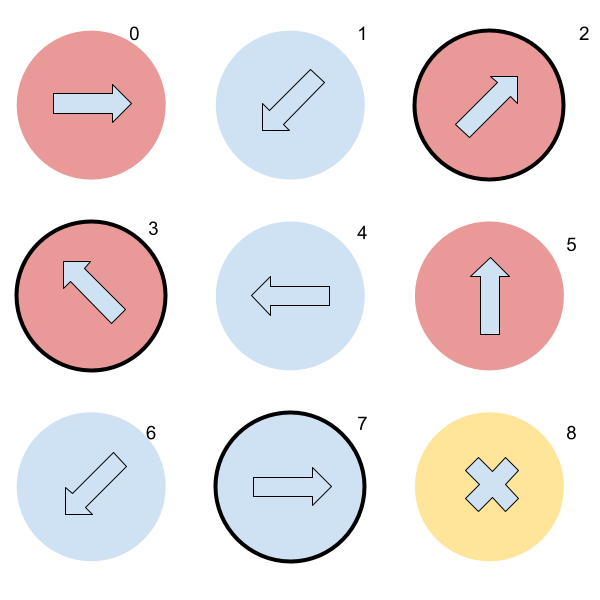
\includegraphics[width=5in]{examplemaze.png}

    \textbf{Figure 1:} Example maze with a few circled nodes,\\
    each labeled with their index.

    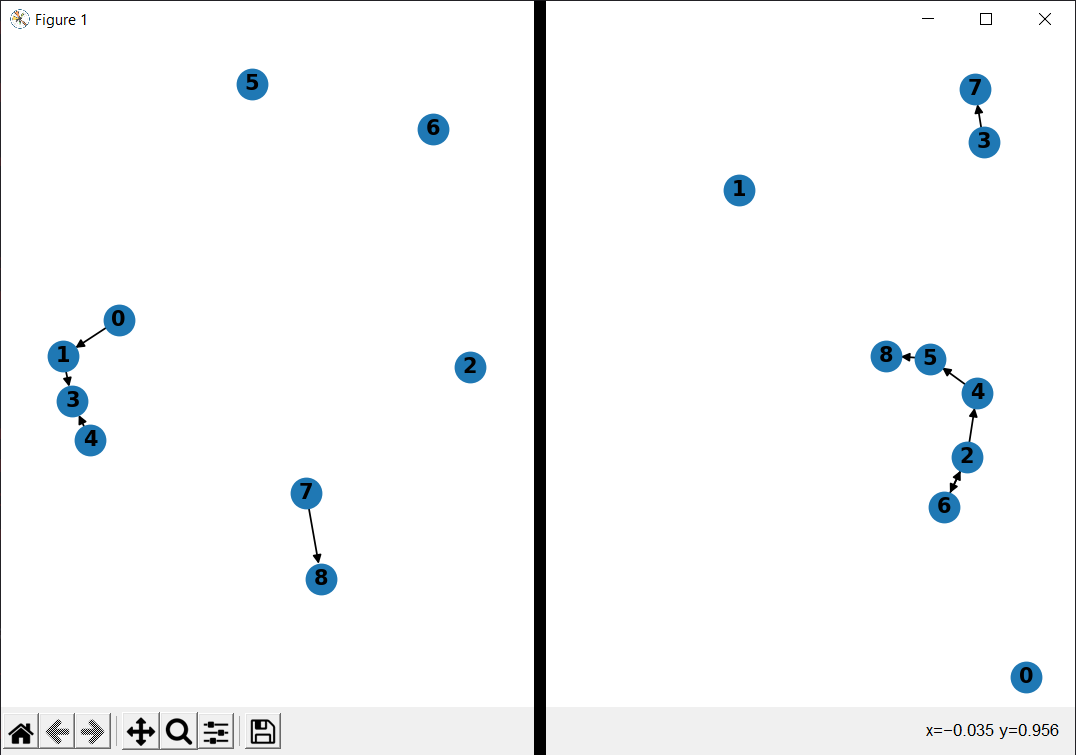
\includegraphics[width=5in]{graphs.png}

    \textbf{Figure 2:} The graphs generated by the Python package 
    \emph{networkx}.\\On the left is the forward-moving edges and the
    right backwards.
\end{center}

Using this model for the problem, we can apply a breadth-first search algorithm
to find the shortest path through the maze. We can convince ourselves this is
the case by imagining these graphs were connected together between circled nodes
in the two graphs. Therefore, each time the BFS gets to a circled node, it
traverses the edge between the graph, effectively switching between the circles
and moving backwards, and the regular forward motion. The algorithm will find a
path if one exists within the maze by exhaustively searching each node but
ensuring that nodes are not repeated.

\section{Code}

\section{Results}

\end{document} 
